
\documentclass[11pt]{article}
\usepackage[margin=1in]{geometry}
\usepackage{graphicx}
\usepackage{booktabs}
\usepackage{longtable}
\usepackage{hyperref}
\title{Dagua Exhaustive Glossary and Reference}
\date{Generated automatically}
\begin{document}
\maketitle
\tableofcontents
\paragraph{Generation note.} This reference was generated from the codebase,
curated glossary metadata, and scripted visuals. Sample visuals use
30 layout steps to keep rebuilds practical.
\section{Basics and Terminology}
\begin{description}\item[DAG] Directed acyclic graph. Edges encode direction, and there are no directed cycles.\item[Rank] A layer index assigned during hierarchical layout. Nodes in the same rank are peers.\item[Cluster] A visual grouping box around related nodes, optionally nested.\item[Port] The attachment location where an edge exits or enters a node.\item[Routing] The post-layout step that turns node positions into edge curves.\item[Projection] A hard corrective step used to enforce constraints like overlap removal or pins.\item[Coarsening] Compression of the graph into a smaller hierarchy level before layout.\item[Prolongation] Expansion of a coarse solution back to a finer graph level.\item[Refinement] Short optimization passes applied after prolongation.\item[Flex] A soft target with a weight that biases layout without forcing a hard lock.\item[Pin] A node position target, usually hard when weight is infinite.\item[Tier-1 metric] A metric cheap enough to compute routinely at any scale.\item[Tier-2 metric] A sampled or costlier metric used when feasible.\item[Tier-3 metric] A hierarchy- or DAG-specific metric that relies on structural metadata.\end{description}\section{Optimization Stages}
\begin{description}\item[Graph Construction] Nodes, edges, labels, clusters, and styles are assembled into a DaguaGraph.\item[Node Sizing] Text measurement and padding determine node bounding boxes before layout.\item[Layering] Topological depth is converted into ordered ranks consistent with graph direction.\item[Coarsening] Large graphs are compressed into smaller layer-aware hierarchy levels.\item[Coarse Optimization] The smallest hierarchy level is optimized first to establish global structure.\item[Prolongation + Refinement] The coarse layout is expanded and refined level by level.\item[Edge Routing] Node positions are converted into routed edge curves and ports.\item[Edge Optimization] Bezier control points are refined to improve crossings and curvature.\item[Label Placement] Edge labels are placed after routing to avoid collisions where possible.\item[Rendering] Nodes, clusters, edges, and labels are turned into raster/vector output.\end{description}\section{Public API Functions}
\begin{longtable}{p{0.22\linewidth}p{0.73\linewidth}}\toprule Name & Signature and summary \\ \midruleanimate & \texttt{animate(graph, config: 'Optional[LayoutConfig]' = None, output: 'Optional[str]' = None, animation\_config: 'Optional[AnimationConfig]' = None, **kwargs) -> 'AnimationResult'}\\Render a faithful optimization animation after layout completes. \\border\_from\_fill & \texttt{border\_from\_fill(fill\_hex: 'str', darken: 'float' = 0.5) -> 'str'}\\Derive border color by darkening the fill in HSL lightness space. \\configure & \texttt{configure(**kwargs: 'Any') -> 'None'}\\Set global defaults via flat namespace. \\configure\_image\_ai & \texttt{configure\_image\_ai(provider: 'Optional[str]' = None, api\_key: 'Optional[str]' = None, api\_key\_env: 'Optional[str]' = None, model: 'Optional[str]' = None, base\_url: 'Optional[str]' = None) -> 'ImageAIConfig'}\\Set process-wide defaults for image-to-graph/theme AI calls. \\defaults & \texttt{defaults(**kwargs: 'Any') -> 'Iterator[None]'}\\Context manager for scoped default overrides. \\draw & \texttt{draw(graph: Any, config: Optional[dagua.config.LayoutConfig] = None, output: Optional[str] = None, relayout: Optional[bool] = None, use\_cached: bool = False, direction: Optional[str] = None, backend: Optional[str] = None, **kwargs: Any) -> Tuple[Any, Any]}\\Layout and render a graph in one convenience call. \\evaluate & \texttt{evaluate(graph: "'DaguaGraph'", positions: 'torch.Tensor', tier: 'str' = 'auto') -> 'Dict[str, float]'}\\Compute layout quality metrics for a graph and position tensor. \\export\_config & \texttt{export\_config(path: 'str') -> 'None'}\\Dump current defaults to a YAML or JSON file. \\from\_dot & \texttt{from\_dot(dot\_string: 'str', **kwargs) -> "'DaguaGraph'"}\\Build a DaguaGraph from a DOT string. \\from\_igraph & \texttt{from\_igraph(ig\_graph, **kwargs) -> "'DaguaGraph'"}\\Build a DaguaGraph from an igraph.Graph. \\from\_image & \texttt{from\_image(image\_path: 'Union[str, Path]', provider: 'Optional[str]' = None, model: 'Optional[str]' = None, *, api\_key: 'Optional[str]' = None, api\_key\_env: 'Optional[str]' = None, base\_url: 'Optional[str]' = None, config: 'Optional[ImageAIConfig]' = None) -> "'DaguaGraph'"}\\Construct a DaguaGraph from an image using an LLM. \\from\_scipy & \texttt{from\_scipy(adj\_matrix, labels=None, **kwargs) -> "'DaguaGraph'"}\\Build a DaguaGraph from a scipy sparse adjacency matrix. \\get\_default\_backend & \texttt{get\_default\_backend() -> 'str'}\\Return the current default render backend. \\get\_defaults & \texttt{get\_defaults() -> 'Dict[str, Any]'}\\Return the current effective defaults as a flat dict. \\get\_image\_ai\_config & \texttt{get\_image\_ai\_config() -> 'ImageAIConfig'}\\Return the current process-wide image AI configuration. \\get\_theme & \texttt{get\_theme(name: 'str') -> 'Theme'}\\Look up a built-in theme by name. Returns a deep copy. \\graph\_code\_from\_image & \texttt{graph\_code\_from\_image(image\_path: 'Union[str, Path]', provider: 'Optional[str]' = None, model: 'Optional[str]' = None, *, api\_key: 'Optional[str]' = None, api\_key\_env: 'Optional[str]' = None, base\_url: 'Optional[str]' = None, config: 'Optional[ImageAIConfig]' = None, function\_name: 'str' = 'build\_graph', include\_demo\_script: 'bool' = False, output\_path: 'str' = 'graph.png') -> 'str'}\\Return canonical Dagua code reconstructed from an image. \\graph\_dict\_from\_image & \texttt{graph\_dict\_from\_image(image\_path: 'Union[str, Path]', provider: 'Optional[str]' = None, model: 'Optional[str]' = None, *, api\_key: 'Optional[str]' = None, api\_key\_env: 'Optional[str]' = None, base\_url: 'Optional[str]' = None, config: 'Optional[ImageAIConfig]' = None) -> 'Dict[str, Any]'}\\Extract a graph JSON dict from an image using a configured AI provider. \\graph\_from\_json & \texttt{graph\_from\_json(data: 'Union[Dict, str, Path]') -> "'DaguaGraph'"}\\Build a DaguaGraph from JSON data. \\graph\_from\_yaml & \texttt{graph\_from\_yaml(data: 'Union[str, Path]') -> "'DaguaGraph'"}\\Build a DaguaGraph from YAML data. \\graph\_script\_from\_dict & \texttt{graph\_script\_from\_dict(graph\_dict: 'Dict[str, Any]', function\_name: 'str' = 'build\_graph', output\_path: 'str' = 'graph.png') -> 'str'}\\Return a ready-to-run Dagua script with layout and export included. \\graph\_to\_json & \texttt{graph\_to\_json(graph: "'DaguaGraph'") -> 'Dict[str, Any]'}\\Serialize a DaguaGraph to a JSON-compatible dict. \\graph\_to\_yaml & \texttt{graph\_to\_yaml(graph: "'DaguaGraph'", path: 'Optional[Union[str, Path]]' = None) -> 'str'}\\Serialize a DaguaGraph to YAML. \\launch\_playground & \texttt{launch\_playground(*, device: 'str' = 'cpu', max\_nodes: 'int' = 2000, animation\_frames: 'int' = 6) -> 'Any'}\\Return an interactive widget for exploring layout parameter intuition. \\layout & \texttt{layout(graph: 'Any', config: 'Optional[LayoutConfig]' = None, trace: 'Any' = None) -> 'torch.Tensor'}\\Compute layout positions for all nodes. \\layout\_all & \texttt{layout\_all(graph: "'DaguaGraph'", engines: 'Optional[List[str]]' = None, timeout: 'float' = 300.0) -> 'Dict[str, Optional[torch.Tensor]]'}\\Run all available competitor engines on a single graph. \\layout\_similarity & \texttt{layout\_similarity(pos\_a: 'torch.Tensor', pos\_b: 'torch.Tensor', edge\_index: 'Optional[torch.Tensor]' = None, k: 'int' = 5) -> 'Dict[str, float]'}\\Compare two layouts of the same graph up to rigid transforms. \\load & \texttt{load(source: 'Union[Dict, str, Path]') -> "'DaguaGraph'"}\\Load a DaguaGraph from a file (YAML/JSON), dict, or string. \\load\_style & \texttt{load\_style(path: 'Union[str, Path]') -> 'Dict[str, Any]'}\\Load a style-only file (YAML/JSON) into a dict. \\make\_fill & \texttt{make\_fill(base\_hex: 'str', bg\_hex: 'str' = '\#FAFAFA', blend: 'float' = 0.25) -> 'str'}\\Blend base color toward background for a muted fill. \\place\_edge\_labels & \texttt{place\_edge\_labels(curves: 'List[BezierCurve]', positions: 'torch.Tensor', node\_sizes: 'torch.Tensor', edge\_labels: 'List[Optional[str]]', graph: 'Optional[Any]' = None) -> 'List[Optional[Tuple[float, float]]]'}\\Compute collision-avoiding positions for edge labels. \\poster & \texttt{poster(graph, positions: 'Optional[torch.Tensor]' = None, config: 'Optional[LayoutConfig]' = None, output: 'Optional[str]' = None, poster\_config: 'Optional[PosterConfig]' = None, **kwargs) -> 'PosterResult'}\\Render a single cinematic still, with LOD support for huge graphs. \\render & \texttt{render(graph: 'Any', positions: 'Any' = None, config: 'Any' = None, output: 'Optional[Union[str, Path]]' = None, format: 'Optional[str]' = None, figsize: 'Optional[Tuple[float, float]]' = None, dpi: 'Optional[int]' = None, show: 'bool' = False, title: 'Optional[str]' = None, curves: 'Optional[List[BezierCurve]]' = None, label\_positions: 'Optional[List[Optional[Tuple[float, float]]]]' = None, svg\_hover\_text: 'bool' = True, backend: 'Optional[str]' = None, fit\_to\_canvas: 'Union[bool, float]' = False, bit\_equivalent: 'bool' = False) -> 'Tuple[Any, Any]'}\\Render a graph with computed node positions. \\reset & \texttt{reset() -> 'None'}\\Restore all defaults to library initial state. \\route\_edges & \texttt{route\_edges(positions: 'torch.Tensor', edge\_index: 'torch.Tensor', node\_sizes: 'torch.Tensor', direction: 'str' = 'TB', graph: 'Optional[Any]' = None) -> 'List[BezierCurve]'}\\Compute routed edge curves for a laid-out graph. \\save & \texttt{save(graph: "'DaguaGraph'", path: 'Union[str, Path]', format: 'Optional[str]' = None) -> 'None'}\\Save a DaguaGraph to a file (YAML or JSON). \\save\_style & \texttt{save\_style(config: 'Dict[str, Any]', path: 'Union[str, Path]') -> 'None'}\\Save a style dict to a YAML/JSON file. \\set\_default\_backend & \texttt{set\_default\_backend(name: 'Optional[str]') -> 'None'}\\Override the global default render backend. \\set\_device & \texttt{set\_device(device: 'str') -> 'None'}\\Set the global default device ('cpu' or 'cuda'). \\set\_theme & \texttt{set\_theme(name: 'str') -> 'None'}\\Set the global default theme by name. \\theme\_code\_from\_image & \texttt{theme\_code\_from\_image(image\_path: 'Union[str, Path]', provider: 'Optional[str]' = None, model: 'Optional[str]' = None, *, api\_key: 'Optional[str]' = None, api\_key\_env: 'Optional[str]' = None, base\_url: 'Optional[str]' = None, config: 'Optional[ImageAIConfig]' = None, variable\_name: 'str' = 'theme') -> 'str'}\\Return canonical Dagua theme code reconstructed from an image. \\theme\_dict\_from\_image & \texttt{theme\_dict\_from\_image(image\_path: 'Union[str, Path]', provider: 'Optional[str]' = None, model: 'Optional[str]' = None, *, api\_key: 'Optional[str]' = None, api\_key\_env: 'Optional[str]' = None, base\_url: 'Optional[str]' = None, config: 'Optional[ImageAIConfig]' = None) -> 'Dict[str, Any]'}\\Extract a theme JSON dict from an image using a configured AI provider. \\theme\_from\_image & \texttt{theme\_from\_image(image\_path: 'Union[str, Path]', provider: 'Optional[str]' = None, model: 'Optional[str]' = None, *, api\_key: 'Optional[str]' = None, api\_key\_env: 'Optional[str]' = None, base\_url: 'Optional[str]' = None, config: 'Optional[ImageAIConfig]' = None) -> 'Theme'}\\Extract a visual theme from a graph image using an LLM. \\to\_igraph & \texttt{to\_igraph(graph: "'DaguaGraph'") -> 'Any'}\\Export a DaguaGraph to an igraph.Graph. \\to\_networkx & \texttt{to\_networkx(graph: "'DaguaGraph'") -> 'Any'}\\Export a DaguaGraph to a NetworkX DiGraph. \\to\_pyg & \texttt{to\_pyg(graph: "'DaguaGraph'") -> 'Any'}\\Export a DaguaGraph to a torch\_geometric.data.Data object. \\to\_scipy & \texttt{to\_scipy(graph: "'DaguaGraph'") -> 'Any'}\\Export a DaguaGraph to a scipy.sparse.csr\_matrix adjacency matrix. \\tour & \texttt{tour(graph, positions: 'Optional[torch.Tensor]' = None, config: 'Optional[LayoutConfig]' = None, output: 'Optional[str]' = None, tour\_config: 'Optional[TourConfig]' = None, **kwargs) -> 'AnimationResult'}\\Render a cinematic tour of the final or current graph layout. \\\bottomrule\end{longtable}\section{Graph Construction and Orchestration Methods}\begin{longtable}{p{0.24\linewidth}p{0.71\linewidth}}\toprule Method & Signature and summary \\ \midruleadd\_cluster & \texttt{add\_cluster(self, name: 'str', members: 'Union[List[Any], Dict]', style: 'Optional[ClusterStyle]' = None, label: 'Optional[str]' = None, parent: 'Optional[str]' = None, strict: 'bool' = True) -> 'None'}\\Add a cluster. Members can be node IDs/indices or nested dict. \\add\_edge & \texttt{add\_edge(self, source: 'Any', target: 'Any', label: 'Optional[str]' = None, type: 'str' = 'normal', style: 'Optional[EdgeStyle]' = None, weight: 'Optional[float]' = None) -> 'None'}\\Add an edge between two nodes. \\add\_node & \texttt{add\_node(self, node\_id: 'Any', label: 'Optional[str]' = None, type: 'str' = 'default', style: 'Optional[NodeStyle]' = None) -> 'int'}\\Add a node and return its integer index. \\align & \texttt{align(self, node\_ids: 'List[Any]', axis: 'str' = 'x', weight: 'float' = 5.0) -> 'None'}\\Align a group of nodes on an axis. \\cache\_layout & \texttt{cache\_layout(self, positions: 'torch.Tensor') -> 'torch.Tensor'}\\Cache positions as the current fresh layout. \\cache\_routing & \texttt{cache\_routing(self, curves, label\_positions: 'Optional[List[Optional[Tuple[float, float]]]]' = None) -> 'None'}\\Cache routed edges and optional label positions for the current revision. \\cluster & \texttt{cluster(self, name: 'str') -> "'ClusterView'"}\\Return a cluster view by name. \\cluster\_children & \texttt{cluster\_children(self, name: 'str') -> 'List[str]'}\\Return direct children of a cluster. \\cluster\_depth & \texttt{cluster\_depth(self, name: 'str') -> 'int'}\\Walk parent chain, return number of hops (0 = root-level cluster). \\clusters\_for\_node & \texttt{clusters\_for\_node(self, node: 'Any') -> "list['ClusterView']"}\\Return all clusters containing a node. \\compute\_node\_sizes & \texttt{compute\_node\_sizes(self, font\_family: 'str' = '', font\_size: 'float' = 8.5) -> 'None'}\\Compute node sizes from labels if not already cached. \\configure & \texttt{configure(self, **kwargs: 'Any') -> 'None'}\\Set graph-scoped style defaults from flat keyword arguments. \\edge & \texttt{edge(self, index: 'int') -> "'EdgeView'"}\\Return an edge view by integer index. \\edges\_between & \texttt{edges\_between(self, source: 'Any', target: 'Any') -> "list['EdgeView']"}\\Return all directed edges from ``source`` to ``target``. \\edges\_for\_node & \texttt{edges\_for\_node(self, node: 'Any') -> "list['EdgeView']"}\\Return all edges incident to a node. \\export\_style & \texttt{export\_style(self, path: 'str') -> 'None'}\\Export this graph's style settings to a YAML/JSON file. \\get\_style\_for\_cluster & \texttt{get\_style\_for\_cluster(self, name: 'str') -> 'ClusterStyle'}\\Get effective style for a cluster. \\get\_style\_for\_edge & \texttt{get\_style\_for\_edge(self, idx: 'int') -> 'EdgeStyle'}\\Get effective style for an edge via 5-level cascade. \\get\_style\_for\_node & \texttt{get\_style\_for\_node(self, idx: 'int') -> 'NodeStyle'}\\Get effective style for a node via 5-level cascade. \\invalidate\_layout & \texttt{invalidate\_layout(self) -> 'None'}\\Drop cached layout-derived artifacts. \\leaf\_cluster\_members & \texttt{leaf\_cluster\_members(self, name: 'str') -> 'List[int]'}\\Recursively collect all leaf node indices (own members + children's members). \\node & \texttt{node(self, id\_or\_index: 'Any') -> "'NodeView'"}\\Return a node view by user ID or integer index. \\node\_id & \texttt{node\_id(self, index: 'int') -> 'Any'}\\Return the user-provided ID for a node index. \\pin & \texttt{pin(self, node\_id: 'Any', x: 'Optional[float]' = None, y: 'Optional[float]' = None, weight: 'float' = inf) -> 'None'}\\Pin a node's position (soft or hard). \\save & \texttt{save(self, path, format=None)}\\Save graph to file (YAML/JSON). Format auto-detected from extension. \\set\_back\_edge\_mask & \texttt{set\_back\_edge\_mask(self, mask: 'torch.Tensor') -> 'None'}\\Manually override which edges are back edges. \\to & \texttt{to(self, device: 'str') -> 'DaguaGraph'}\\Move graph tensors to a device. \\to\_igraph & \texttt{to\_igraph(self)}\\Export to igraph.Graph. See ``dagua.io.to\_igraph``. \\to\_json & \texttt{to\_json(self) -> 'Dict[str, Any]'}\\Serialize this graph to a JSON-compatible dict. \\to\_networkx & \texttt{to\_networkx(self)}\\Export to NetworkX DiGraph. See ``dagua.io.to\_networkx``. \\to\_pyg & \texttt{to\_pyg(self)}\\Export to torch\_geometric.data.Data. See ``dagua.io.to\_pyg``. \\to\_scipy & \texttt{to\_scipy(self)}\\Export to scipy.sparse.csr\_matrix. See ``dagua.io.to\_scipy``. \\to\_yaml & \texttt{to\_yaml(self, path=None) -> 'str'}\\Serialize to YAML string (or write to file if path given). \\\bottomrule\end{longtable}\section{Configs and Data Structures}\subsection{LayoutConfig}All tunable parameters for the layout engine.\begin{longtable}{p{0.24\linewidth}p{0.24\linewidth}p{0.18\linewidth}p{0.26\linewidth}}\toprule Field & Type & Default & Notes \\ \midrulequality & Union[float, str] & \texttt{'balanced'} & LayoutConfig field \\time\_budget\_s & Optional[float] & \texttt{None} & LayoutConfig field \\node\_sep & float & \texttt{70.0} & LayoutConfig field \\rank\_sep & float & \texttt{240.0} & LayoutConfig field \\direction & str & \texttt{'TB'} & LayoutConfig field \\steps & int & \texttt{0} & LayoutConfig field \\lr & float & \texttt{0.05} & LayoutConfig field \\device & str & \texttt{'cpu'} & LayoutConfig field \\seed & Optional[int] & \texttt{42} & LayoutConfig field \\fidelity\_dtype & Optional[torch.dtype] & \texttt{None} & LayoutConfig field \\multi\_start\_k & int & \texttt{1} & LayoutConfig field \\route\_flat\_to\_stress & bool & \texttt{True} & LayoutConfig field \\force\_pipeline & Optional[Literal['tree', 'layered\_dag', 'force\_directed', 'hybrid', 'hybrid\_v2', 'planar', 'stress', 'legacy\_monolith']] & \texttt{None} & LayoutConfig field \\edge\_equalize\_polish & bool & \texttt{True} & LayoutConfig field \\try\_planar\_first & bool & \texttt{False} & LayoutConfig field \\adaptive\_spacing & bool & \texttt{True} & LayoutConfig field \\verbose & bool & \texttt{False} & LayoutConfig field \\w\_dag & float & \texttt{10.0} & LayoutConfig field \\w\_attract & float & \texttt{2.0} & LayoutConfig field \\w\_attract\_x\_bias & float & \texttt{1.0} & LayoutConfig field \\w\_repel & float & \texttt{0.2} & LayoutConfig field \\w\_overlap & float & \texttt{5.0} & LayoutConfig field \\w\_cluster & float & \texttt{1.0} & LayoutConfig field \\w\_cluster\_contain & float & \texttt{2.0} & LayoutConfig field \\cluster\_aware & bool & \texttt{True} & LayoutConfig field \\cluster\_side\_padding\_pt & float & \texttt{8.0} & LayoutConfig field \\cluster\_label\_band\_pt & float & \texttt{26.0} & LayoutConfig field \\cluster\_external\_clearance\_pt & float & \texttt{10.0} & LayoutConfig field \\w\_align & float & \texttt{5.0} & LayoutConfig field \\w\_crossing & float & \texttt{1.8} & LayoutConfig field \\w\_straightness & float & \texttt{0.5} & LayoutConfig field \\w\_length\_variance & float & \texttt{8.0} & LayoutConfig field \\w\_stress & float & \texttt{0.0} & LayoutConfig field \\w\_stress\_n\_pivots & int & \texttt{50} & LayoutConfig field \\w\_spacing & float & \texttt{0.3} & LayoutConfig field \\w\_fanout & float & \texttt{0.3} & LayoutConfig field \\w\_back\_edge & float & \texttt{0.3} & LayoutConfig field \\exact\_repulsion & bool & \texttt{False} & LayoutConfig field \\exact\_repulsion\_threshold & int & \texttt{500} & LayoutConfig field \\negative\_sample\_k & int & \texttt{128} & LayoutConfig field \\use\_tree\_fast\_path & bool & \texttt{False} & LayoutConfig field \\use\_native\_median\_transpose & bool & \texttt{True} & LayoutConfig field \\native\_median\_passes & int & \texttt{4} & LayoutConfig field \\native\_transpose\_passes & int & \texttt{8} & LayoutConfig field \\brandes\_koepf\_refine & bool & \texttt{True} & LayoutConfig field \\layered\_rank\_row\_snap & bool & \texttt{True} & LayoutConfig field \\cluster\_aware\_x\_compaction & bool & \texttt{True} & LayoutConfig field \\tiny\_multiedge\_rank\_sep\_cap & bool & \texttt{True} & LayoutConfig field \\tiny\_multiedge\_rank\_sep\_max & float & \texttt{240.0} & LayoutConfig field \\insert\_dummy\_nodes & bool & \texttt{True} & LayoutConfig field \\decompose\_components & bool & \texttt{True} & LayoutConfig field \\component\_tiling\_crossing\_risk & bool & \texttt{True} & LayoutConfig field \\multilevel\_threshold & int & \texttt{20000} & LayoutConfig field \\multilevel\_min\_nodes & int & \texttt{2000} & LayoutConfig field \\multilevel\_coarse\_steps & int & \texttt{100} & LayoutConfig field \\multilevel\_refine\_steps & int & \texttt{25} & LayoutConfig field \\rvs\_threshold & int & \texttt{100000} & LayoutConfig field \\rvs\_nn\_k & int & \texttt{20} & LayoutConfig field \\per\_loss\_backward & str & \texttt{'auto'} & LayoutConfig field \\gradient\_checkpointing & str & \texttt{'auto'} & LayoutConfig field \\hybrid\_device & str & \texttt{'auto'} & LayoutConfig field \\execution\_mode & Literal['auto', 'standard', 'subset\_gpu'] & \texttt{'auto'} & LayoutConfig field \\subset\_gpu\_threshold & int & \texttt{10000000} & LayoutConfig field \\optimizer\_fallback & Literal['auto', 'adam', 'sgd'] & \texttt{'auto'} & LayoutConfig field \\num\_workers & int & \texttt{0} & LayoutConfig field \\edge\_batch\_size & int & \texttt{0} & LayoutConfig field \\overlap\_check\_interval & int & \texttt{0} & LayoutConfig field \\repel\_amortize\_interval & int & \texttt{2} & LayoutConfig field \\repel\_amortize\_threshold & int & \texttt{10000000} & LayoutConfig field \\fanout\_amortize\_interval & int & \texttt{3} & LayoutConfig field \\fanout\_amortize\_threshold & int & \texttt{10000000} & LayoutConfig field \\edge\_random\_fraction & float & \texttt{0.2} & LayoutConfig field \\relax\_steps & int & \texttt{0} & LayoutConfig field \\offload\_to\_disk & bool & \texttt{True} & LayoutConfig field \\flex & Optional['LayoutFlex'] & \texttt{None} & LayoutConfig field \\edge\_opt\_steps & int & \texttt{0} & LayoutConfig field \\edge\_opt\_lr & float & \texttt{0.1} & LayoutConfig field \\edge\_routing & str & \texttt{'differentiable'} & LayoutConfig field \\edge\_routing\_auto\_skip\_threshold & int & \texttt{5} & LayoutConfig field \\w\_edge\_crossing & float & \texttt{0.5} & LayoutConfig field \\w\_edge\_node\_crossing & float & \texttt{10.0} & LayoutConfig field \\w\_edge\_angular\_res & float & \texttt{0.0} & LayoutConfig field \\w\_edge\_curvature\_consistency & float & \texttt{0.0} & LayoutConfig field \\w\_edge\_curvature\_penalty & float & \texttt{1.0} & LayoutConfig field \\w\_edge\_cluster\_crossing & float & \texttt{4.0} & LayoutConfig field \\use\_pipeline & bool & \texttt{False} & LayoutConfig field \\algorithm & Optional[str] & \texttt{None} & LayoutConfig field \\algorithm\_params & dict[str, Any] & \texttt{dict()} & LayoutConfig field \\\bottomrule\end{longtable}\subsection{NodeStyle}Visual style for a node.\begin{longtable}{p{0.24\linewidth}p{0.24\linewidth}p{0.18\linewidth}p{0.26\linewidth}}\toprule Field & Type & Default & Notes \\ \midruleshape & str & \texttt{'roundrect'} & NodeStyle field \\fill & str & \texttt{''} & NodeStyle field \\stroke & str & \texttt{''} & NodeStyle field \\stroke\_width & float & \texttt{0.57} & NodeStyle field \\stroke\_width\_override\_points & Optional[float] & \texttt{None} & NodeStyle field \\stroke\_dash & str & \texttt{'solid'} & NodeStyle field \\stroke\_dash\_pattern & Optional[Tuple[float, ...]] & \texttt{None} & NodeStyle field \\border\_opacity & float & \texttt{1.0} & NodeStyle field \\font\_family & str & \texttt{''} & NodeStyle field \\font\_size & float & \texttt{9.0} & NodeStyle field \\font\_size\_override\_points & Optional[float] & \texttt{None} & NodeStyle field \\font\_color & str & \texttt{'\#2D2D2D'} & NodeStyle field \\text\_align & str & \texttt{'center'} & NodeStyle field \\text\_valign & str & \texttt{'center'} & NodeStyle field \\text\_rotation & float & \texttt{0.0} & NodeStyle field \\text\_wrap & str & \texttt{'none'} & NodeStyle field \\text\_max\_width & Optional[float] & \texttt{None} & NodeStyle field \\text\_transform & str & \texttt{'none'} & NodeStyle field \\text\_outline & bool & \texttt{False} & NodeStyle field \\text\_outline\_color & str & \texttt{'\#FFFFFF'} & NodeStyle field \\text\_outline\_width & float & \texttt{1.4} & NodeStyle field \\text\_background & str & \texttt{''} & NodeStyle field \\text\_background\_opacity & float & \texttt{0.85} & NodeStyle field \\text\_background\_padding & Tuple[float, float] & \texttt{(3.0, 2.0)} & NodeStyle field \\text\_background\_corner\_radius & float & \texttt{2.0} & NodeStyle field \\external\_label & str & \texttt{''} & NodeStyle field \\external\_label\_position & str & \texttt{'bottom'} & NodeStyle field \\external\_label\_font\_size & float & \texttt{8.0} & NodeStyle field \\external\_label\_font\_color & str & \texttt{''} & NodeStyle field \\external\_label\_offset & float & \texttt{4.0} & NodeStyle field \\padding & Tuple[float, float] & \texttt{(11.0, 9.0)} & NodeStyle field \\corner\_radius & Union[float, Tuple[float, float, float, float]] & \texttt{6.0} & NodeStyle field \\scale\_corner\_radius & bool & \texttt{False} & NodeStyle field \\opacity & float & \texttt{1.0} & NodeStyle field \\gradient & str & \texttt{'none'} & NodeStyle field \\gradient\_color & str & \texttt{''} & NodeStyle field \\gradient\_angle & float & \texttt{0.0} & NodeStyle field \\base\_color & str & \texttt{'\#56B4E9'} & NodeStyle field \\font\_weight & str & \texttt{'regular'} & NodeStyle field \\font\_style & str & \texttt{'normal'} & NodeStyle field \\shadow & bool & \texttt{False} & NodeStyle field \\shadow\_offset & Tuple[float, float] & \texttt{(1.5, -1.5)} & NodeStyle field \\shadow\_color & str & \texttt{'\#00000020'} & NodeStyle field \\shadow\_blur & float & \texttt{0.0} & NodeStyle field \\min\_width & Optional[float] & \texttt{None} & NodeStyle field \\min\_height & Optional[float] & \texttt{None} & NodeStyle field \\auto\_size\_to\_label & bool & \texttt{False} & NodeStyle field \\aspect\_ratio & Optional[float] & \texttt{None} & NodeStyle field \\overflow\_policy & str & \texttt{'shrink\_text'} & NodeStyle field \\min\_font\_size & float & \texttt{5.0} & NodeStyle field \\auto\_expand\_on\_floor\_overflow & bool & \texttt{True} & NodeStyle field \\label\_format & str & \texttt{'plain'} & NodeStyle field \\border\_count & int & \texttt{1} & NodeStyle field \\border\_position & str & \texttt{'center'} & NodeStyle field \\stroke\_cap & str & \texttt{'butt'} & NodeStyle field \\stroke\_join & str & \texttt{'miter'} & NodeStyle field \\fill\_pattern & str & \texttt{'solid'} & NodeStyle field \\fill\_pattern\_colors & Optional[List[str]] & \texttt{None} & NodeStyle field \\fill\_pattern\_values & Optional[List[float]] & \texttt{None} & NodeStyle field \\fill\_pattern\_angle & float & \texttt{0.0} & NodeStyle field \\fill\_pattern\_hole & float & \texttt{0.0} & NodeStyle field \\image & str & \texttt{''} & NodeStyle field \\image\_fit & str & \texttt{'contain'} & NodeStyle field \\image\_opacity & float & \texttt{1.0} & NodeStyle field \\bevel & bool & \texttt{False} & NodeStyle field \\bevel\_intensity & float & \texttt{0.5} & NodeStyle field \\\bottomrule\end{longtable}\subsection{EdgeStyle}Visual style for an edge.\begin{longtable}{p{0.24\linewidth}p{0.24\linewidth}p{0.18\linewidth}p{0.26\linewidth}}\toprule Field & Type & Default & Notes \\ \midrulecolor & str & \texttt{'\#6B7280'} & EdgeStyle field \\width & float & \texttt{1.4} & EdgeStyle field \\width\_override\_points & Optional[float] & \texttt{None} & EdgeStyle field \\arrow & str & \texttt{'normal'} & EdgeStyle field \\tail\_arrow & str & \texttt{'none'} & EdgeStyle field \\arrow\_fill & str & \texttt{'filled'} & EdgeStyle field \\arrow\_color & str & \texttt{''} & EdgeStyle field \\arrow\_length & float & \texttt{12.0} & EdgeStyle field \\arrow\_width & float & \texttt{9.0} & EdgeStyle field \\arrowsize & float & \texttt{1.0} & EdgeStyle field \\arrow\_scale & Optional[float] & \texttt{None} & EdgeStyle field \\arrow\_node\_fraction & float & \texttt{0.35} & EdgeStyle field \\arrow\_width\_ratio & float & \texttt{0.85} & EdgeStyle field \\style & str & \texttt{'solid'} & EdgeStyle field \\line\_cap & str & \texttt{'butt'} & EdgeStyle field \\line\_join & str & \texttt{'miter'} & EdgeStyle field \\opacity & float & \texttt{0.75} & EdgeStyle field \\routing & str & \texttt{'bezier'} & EdgeStyle field \\label\_font\_size & float & \texttt{7.0} & EdgeStyle field \\font\_size\_override\_points & Optional[float] & \texttt{None} & EdgeStyle field \\label\_font\_color & str & \texttt{'\#2D2D2D'} & EdgeStyle field \\label\_background & str & \texttt{'\#FAFAFA'} & EdgeStyle field \\label\_background\_opacity & float & \texttt{0.85} & EdgeStyle field \\label\_background\_padding & Tuple[float, float] & \texttt{(3.0, 2.0)} & EdgeStyle field \\label\_background\_corner\_radius & float & \texttt{2.0} & EdgeStyle field \\label\_font\_family & str & \texttt{''} & EdgeStyle field \\label\_font\_weight & str & \texttt{'regular'} & EdgeStyle field \\label\_position & float & \texttt{0.5} & EdgeStyle field \\label\_offset & float & \texttt{8.0} & EdgeStyle field \\label\_side & str & \texttt{'auto'} & EdgeStyle field \\curvature & float & \texttt{0.4} & EdgeStyle field \\port\_style & str & \texttt{'distributed'} & EdgeStyle field \\label\_avoidance & bool & \texttt{True} & EdgeStyle field \\taper & bool & \texttt{False} & EdgeStyle field \\taper\_width\_start & float & \texttt{3.0} & EdgeStyle field \\taper\_width\_end & float & \texttt{0.5} & EdgeStyle field \\head\_label & str & \texttt{''} & EdgeStyle field \\tail\_label & str & \texttt{''} & EdgeStyle field \\head\_label\_offset & float & \texttt{5.0} & EdgeStyle field \\tail\_label\_offset & float & \texttt{5.0} & EdgeStyle field \\color\_gradient & str & \texttt{'none'} & EdgeStyle field \\color\_gradient\_end & str & \texttt{''} & EdgeStyle field \\crossing\_style & str & \texttt{'none'} & EdgeStyle field \\crossing\_size & float & \texttt{6.0} & EdgeStyle field \\port\_indicator & str & \texttt{'none'} & EdgeStyle field \\port\_indicator\_size & float & \texttt{5.0} & EdgeStyle field \\port\_indicator\_color & str & \texttt{''} & EdgeStyle field \\\bottomrule\end{longtable}\subsection{ClusterStyle}Visual style for a cluster box.\begin{longtable}{p{0.24\linewidth}p{0.24\linewidth}p{0.18\linewidth}p{0.26\linewidth}}\toprule Field & Type & Default & Notes \\ \midrulefill & str & \texttt{'\#F5F5F0'} & ClusterStyle field \\stroke & str & \texttt{'\#D4D4D4'} & ClusterStyle field \\stroke\_width & float & \texttt{0.7} & ClusterStyle field \\stroke\_width\_override\_points & Optional[float] & \texttt{None} & ClusterStyle field \\stroke\_dash & str & \texttt{'solid'} & ClusterStyle field \\corner\_radius & float & \texttt{8.0} & ClusterStyle field \\padding & float & \texttt{38.0} & ClusterStyle field \\label\_position & str & \texttt{'top-left'} & ClusterStyle field \\font\_size & float & \texttt{9.5} & ClusterStyle field \\font\_size\_override\_points & Optional[float] & \texttt{None} & ClusterStyle field \\font\_weight & str & \texttt{'bold'} & ClusterStyle field \\font\_color & str & \texttt{'\#4A4A4A'} & ClusterStyle field \\opacity & float & \texttt{0.32} & ClusterStyle field \\fill\_opacity & Optional[float] & \texttt{None} & ClusterStyle field \\border\_opacity & Optional[float] & \texttt{None} & ClusterStyle field \\label\_background & str & \texttt{''} & ClusterStyle field \\label\_background\_opacity & float & \texttt{0.85} & ClusterStyle field \\label\_background\_padding & Tuple[float, float] & \texttt{(3.0, 2.0)} & ClusterStyle field \\label\_background\_corner\_radius & float & \texttt{2.0} & ClusterStyle field \\font\_family & str & \texttt{''} & ClusterStyle field \\label\_offset & Tuple[float, float] & \texttt{(10.0, 12.0)} & ClusterStyle field \\text\_wrap & str & \texttt{'none'} & ClusterStyle field \\text\_max\_width & Optional[float] & \texttt{None} & ClusterStyle field \\depth\_fill\_step & float & \texttt{0.03} & ClusterStyle field \\depth\_stroke\_step & float & \texttt{0.05} & ClusterStyle field \\depth\_stroke\_width\_step & float & \texttt{0.0} & ClusterStyle field \\depth\_opacity\_step & float & \texttt{-0.05} & ClusterStyle field \\depth\_font\_size\_step & float & \texttt{-0.5} & ClusterStyle field \\depth\_padding\_step & float & \texttt{-3.0} & ClusterStyle field \\depth\_corner\_radius\_step & float & \texttt{0.0} & ClusterStyle field \\font\_size\_scaling & Literal['by\_height', 'fixed'] & \texttt{'by\_height'} & ClusterStyle field \\member\_node\_style & Optional[NodeStyle] & \texttt{None} & ClusterStyle field \\member\_edge\_style & Optional[EdgeStyle] & \texttt{None} & ClusterStyle field \\\bottomrule\end{longtable}\subsection{GraphStyle}Graph-level visual settings (all render-only, no layout effect).\begin{longtable}{p{0.24\linewidth}p{0.24\linewidth}p{0.18\linewidth}p{0.26\linewidth}}\toprule Field & Type & Default & Notes \\ \midrulebackground\_color & str & \texttt{'\#FAFAFA'} & GraphStyle field \\margin & float & \texttt{18.0} & GraphStyle field \\margin\_inches & float & \texttt{0.11} & GraphStyle field \\dpi & int & \texttt{96} & GraphStyle field \\size\_inches & Optional[Tuple[float, float]] & \texttt{None} & GraphStyle field \\size\_force\_fit & bool & \texttt{False} & GraphStyle field \\pad\_inches & float & \texttt{0.0} & GraphStyle field \\ratio & Optional[str] & \texttt{None} & GraphStyle field \\density\_aware\_node\_shrink & bool & \texttt{False} & GraphStyle field \\title\_font\_size & float & \texttt{10.0} & GraphStyle field \\title\_font\_weight & str & \texttt{'regular'} & GraphStyle field \\title\_font\_color & str & \texttt{'\#2D2D2D'} & GraphStyle field \\title\_font\_family & str & \texttt{''} & GraphStyle field \\edge\_label\_font\_size & float & \texttt{7.0} & GraphStyle field \\edge\_label\_background & str & \texttt{'\#FAFAFA'} & GraphStyle field \\edge\_label\_background\_opacity & float & \texttt{0.85} & GraphStyle field \\node\_label\_secondary\_scale & float & \texttt{0.85} & GraphStyle field \\max\_figsize & Tuple[float, float] & \texttt{(30.0, 40.0)} & GraphStyle field \\min\_figsize & Tuple[float, float] & \texttt{(4.0, 3.0)} & GraphStyle field \\\bottomrule\end{longtable}\subsection{AnimationConfig}Animation output and capture controls.\begin{longtable}{p{0.24\linewidth}p{0.24\linewidth}p{0.18\linewidth}p{0.26\linewidth}}\toprule Field & Type & Default & Notes \\ \midrulefps & int & \texttt{20} & AnimationConfig field \\dpi & int & \texttt{140} & AnimationConfig field \\figsize & Optional[Tuple[float, float]] & \texttt{None} & AnimationConfig field \\format & Optional[str] & \texttt{None} & AnimationConfig field \\camera & str & \texttt{'adaptive'} & AnimationConfig field \\center\_on & Optional[Any] & \texttt{None} & AnimationConfig field \\bounds & Optional[Tuple[float, float, float, float]] & \texttt{None} & AnimationConfig field \\follow\_padding & float & \texttt{80.0} & AnimationConfig field \\hold\_start\_frames & int & \texttt{6} & AnimationConfig field \\hold\_end\_frames & int & \texttt{12} & AnimationConfig field \\transition\_frames & int & \texttt{6} & AnimationConfig field \\show\_phase\_cards & bool & \texttt{True} & AnimationConfig field \\max\_layout\_frames & int & \texttt{36} & AnimationConfig field \\max\_edge\_frames & int & \texttt{18} & AnimationConfig field \\overlay\_title & bool & \texttt{True} & AnimationConfig field \\output & Optional[str] & \texttt{None} & AnimationConfig field \\save\_frames\_dir & Optional[str] & \texttt{None} & AnimationConfig field \\codec & str & \texttt{'libx264'} & AnimationConfig field \\bitrate & str & \texttt{'6M'} & AnimationConfig field \\\bottomrule\end{longtable}\subsection{PosterConfig}Single-frame showcase export using the cinematic tour camera logic.\begin{longtable}{p{0.24\linewidth}p{0.24\linewidth}p{0.18\linewidth}p{0.26\linewidth}}\toprule Field & Type & Default & Notes \\ \midruledpi & int & \texttt{220} & PosterConfig field \\figsize & Optional[Tuple[float, float]] & \texttt{None} & PosterConfig field \\format & Optional[str] & \texttt{None} & PosterConfig field \\output & Optional[str] & \texttt{None} & PosterConfig field \\scene & str & \texttt{'auto'} & PosterConfig field \\keyframes & Optional[List['CameraKeyframe']] & \texttt{None} & PosterConfig field \\keyframe\_index & Optional[int] & \texttt{None} & PosterConfig field \\show\_titles & bool & \texttt{True} & PosterConfig field \\follow\_padding & float & \texttt{80.0} & PosterConfig field \\lod\_threshold & int & \texttt{100000} & PosterConfig field \\detail\_node\_limit & int & \texttt{12000} & PosterConfig field \\label\_node\_limit & int & \texttt{160} & PosterConfig field \\edge\_sample\_limit & int & \texttt{60000} & PosterConfig field \\density\_bins & int & \texttt{280} & PosterConfig field \\density\_gamma & float & \texttt{0.52} & PosterConfig field \\\bottomrule\end{longtable}\subsection{TourConfig}Camera tour controls for final/current graph showcases.\begin{longtable}{p{0.24\linewidth}p{0.24\linewidth}p{0.18\linewidth}p{0.26\linewidth}}\toprule Field & Type & Default & Notes \\ \midrulefps & int & \texttt{24} & TourConfig field \\dpi & int & \texttt{160} & TourConfig field \\figsize & Optional[Tuple[float, float]] & \texttt{None} & TourConfig field \\format & Optional[str] & \texttt{None} & TourConfig field \\output & Optional[str] & \texttt{None} & TourConfig field \\scene & str & \texttt{'auto'} & TourConfig field \\keyframes & Optional[List[CameraKeyframe]] & \texttt{None} & TourConfig field \\hold\_start\_frames & int & \texttt{10} & TourConfig field \\hold\_end\_frames & int & \texttt{14} & TourConfig field \\show\_titles & bool & \texttt{True} & TourConfig field \\follow\_padding & float & \texttt{80.0} & TourConfig field \\codec & str & \texttt{'libx264'} & TourConfig field \\bitrate & str & \texttt{'8M'} & TourConfig field \\save\_frames\_dir & Optional[str] & \texttt{None} & TourConfig field \\lod\_threshold & int & \texttt{100000} & TourConfig field \\detail\_node\_limit & int & \texttt{8000} & TourConfig field \\label\_node\_limit & int & \texttt{120} & TourConfig field \\edge\_sample\_limit & int & \texttt{40000} & TourConfig field \\density\_bins & int & \texttt{220} & TourConfig field \\density\_gamma & float & \texttt{0.55} & TourConfig field \\\bottomrule\end{longtable}\subsection{Flex}A soft target value with a weight controlling how strongly the layout\begin{longtable}{p{0.24\linewidth}p{0.24\linewidth}p{0.18\linewidth}p{0.26\linewidth}}\toprule Field & Type & Default & Notes \\ \midruletarget & float & \texttt{<required>} & Flex field \\weight & float & \texttt{1.0} & Flex field \\\bottomrule\end{longtable}\subsection{LayoutFlex}Flex targets for layout-affecting properties.\begin{longtable}{p{0.24\linewidth}p{0.24\linewidth}p{0.18\linewidth}p{0.26\linewidth}}\toprule Field & Type & Default & Notes \\ \midrulenode\_sep & Optional[Flex] & \texttt{None} & LayoutFlex field \\rank\_sep & Optional[Flex] & \texttt{None} & LayoutFlex field \\pins & Optional[Dict[Any, Tuple[Optional[Flex], Optional[Flex]]]] & \texttt{None} & LayoutFlex field \\align\_x & Optional[List[AlignGroup]] & \texttt{None} & LayoutFlex field \\align\_y & Optional[List[AlignGroup]] & \texttt{None} & LayoutFlex field \\\bottomrule\end{longtable}\subsection{AlignGroup}A group of nodes that should share the same position on one axis.\begin{longtable}{p{0.24\linewidth}p{0.24\linewidth}p{0.18\linewidth}p{0.26\linewidth}}\toprule Field & Type & Default & Notes \\ \midrulenodes & List[Any] & \texttt{<required>} & AlignGroup field \\weight & float & \texttt{5.0} & AlignGroup field \\\bottomrule\end{longtable}\section{Loss Functions}\begin{longtable}{p{0.28\linewidth}p{0.67\linewidth}}\toprule Loss & Signature and summary \\ \midrule\_crossing\_loss\_fallback & \texttt{\_crossing\_loss\_fallback(pos: 'torch.Tensor', edge\_index: 'torch.Tensor', alpha: 'float', max\_pairs: 'int') -> 'torch.Tensor'}\\Original crossing proxy for when layer info is unavailable. \\\_crossing\_loss\_layered & \texttt{\_crossing\_loss\_layered(pos: 'torch.Tensor', edge\_index: 'torch.Tensor', alpha: 'float', max\_pairs: 'int', layer\_assignments: 'Union[List[int], torch.Tensor]') -> 'torch.Tensor'}\\Adjacent-layer crossing loss with virtual node decomposition (vectorized). \\\_curvature\_consistency\_loss & \texttt{\_curvature\_consistency\_loss(endpoints: 'torch.Tensor', cp: 'torch.Tensor', t\_samples: 'torch.Tensor') -> 'torch.Tensor'}\\Penalize variance of curvature κ across all edges. \\\_curvature\_penalty\_loss & \texttt{\_curvature\_penalty\_loss(endpoints: 'torch.Tensor', cp: 'torch.Tensor', t\_samples: 'torch.Tensor') -> 'torch.Tensor'}\\Penalize total curvature — prefer straighter paths. \\\_edge\_cluster\_crossing\_loss & \texttt{\_edge\_cluster\_crossing\_loss(points: 'torch.Tensor', cluster\_bboxes: 'torch.Tensor', node\_cluster\_mask: 'torch.Tensor', src\_list: 'list', tgt\_list: 'list', E: 'int') -> 'torch.Tensor'}\\Penalize edge sample points inside foreign cluster bboxes. \\\_edge\_crossing\_loss & \texttt{\_edge\_crossing\_loss(points: 'torch.Tensor', E: 'int') -> 'torch.Tensor'}\\Sigmoid-relaxed edge crossing proxy. \\\_edge\_node\_crossing\_loss & \texttt{\_edge\_node\_crossing\_loss(points: 'torch.Tensor', pos: 'torch.Tensor', sizes: 'torch.Tensor', src\_list: 'list', tgt\_list: 'list', E: 'int') -> 'torch.Tensor'}\\Penalty for edge sample points close to unrelated node bboxes. \\\_port\_angular\_resolution\_loss & \texttt{\_port\_angular\_resolution\_loss(endpoints: 'torch.Tensor', cp: 'torch.Tensor', src\_list: 'list', tgt\_list: 'list') -> 'torch.Tensor'}\\Penalize small angles between incident edges at each node. \\\_rectilinear\_crossing\_loss & \texttt{\_rectilinear\_crossing\_loss(segments: 'torch.Tensor', segment\_edges: 'torch.Tensor') -> 'torch.Tensor'}\\Penalize soft intersections between rectilinear sub-segments. \\\_sampled\_curvature\_consistency\_loss & \texttt{\_sampled\_curvature\_consistency\_loss(points: 'torch.Tensor') -> 'torch.Tensor'}\\Penalize variance in discrete sampled curvature across routes. \\\_sampled\_curvature\_penalty\_loss & \texttt{\_sampled\_curvature\_penalty\_loss(points: 'torch.Tensor') -> 'torch.Tensor'}\\Penalize total discrete sampled curvature. \\\_spacing\_consistency\_loss\_layerlocal & \texttt{\_spacing\_consistency\_loss\_layerlocal(pos: 'torch.Tensor', node\_sizes: 'torch.Tensor', layers: 'torch.Tensor', offsets: 'torch.Tensor', num\_layers: 'int', target\_gap: 'float', device: 'torch.device', layer\_index: 'Optional[LayerIndex]' = None) -> 'torch.Tensor'}\\Layer-local spacing consistency for very large graphs (N > 100M). \\alignment\_loss & \texttt{alignment\_loss(pos: 'torch.Tensor', align\_groups: 'List[Tuple[torch.Tensor, float, int]]') -> 'torch.Tensor'}\\Penalize positional variance within alignment groups. \\back\_edge\_compactness\_loss & \texttt{back\_edge\_compactness\_loss(pos: 'torch.Tensor', edge\_index: 'torch.Tensor', edge\_ctx: 'Optional[EdgeBatchLike]' = None) -> 'torch.Tensor'}\\Penalize horizontal distance in back-edge pairs (target above source). \\cluster\_compactness\_loss & \texttt{cluster\_compactness\_loss(pos: 'torch.Tensor', clusters: 'dict', device: 'torch.device', cache: 'Optional[\_ClusterCache]' = None) -> 'torch.Tensor'}\\Nodes in same cluster attract their cluster centroid (vectorized). \\cluster\_containment\_loss & \texttt{cluster\_containment\_loss(pos: 'torch.Tensor', node\_sizes: 'torch.Tensor', clusters: 'dict', cluster\_parents: 'Dict[str, Optional[str]]', padding: 'float' = 18.0, device: 'Optional[torch.device]' = None, cache: 'Optional[\_ClusterCache]' = None) -> 'torch.Tensor'}\\Child cluster bboxes must stay inside parent cluster bboxes (vectorized). \\cluster\_separation\_loss & \texttt{cluster\_separation\_loss(pos: 'torch.Tensor', node\_sizes: 'torch.Tensor', clusters: 'dict', padding: 'float' = 10.0, device: 'Optional[torch.device]' = None, cluster\_parents: 'Optional[Dict[str, Optional[str]]]' = None, cache: 'Optional[\_ClusterCache]' = None) -> 'torch.Tensor'}\\Sibling cluster bounding boxes repel (vectorized). \\crossing\_loss & \texttt{crossing\_loss(pos: 'torch.Tensor', edge\_index: 'torch.Tensor', alpha: 'float' = 5.0, max\_pairs: 'int' = 2000, layer\_assignments: 'Optional[Union[List[int], torch.Tensor]]' = None) -> 'torch.Tensor'}\\Differentiable crossing proxy using adjacent-layer sigmoid relaxation. \\dag\_ordering\_loss & \texttt{dag\_ordering\_loss(pos: 'torch.Tensor', edge\_index: 'torch.Tensor', node\_sizes: 'torch.Tensor', rank\_sep: 'float' = 50.0, edge\_ctx: 'Optional[EdgeBatchLike]' = None) -> 'torch.Tensor'}\\Penalize edges whose targets drift above their sources. \\edge\_attraction\_loss & \texttt{edge\_attraction\_loss(pos: 'torch.Tensor', edge\_index: 'torch.Tensor', x\_bias: 'float' = 4.0, edge\_ctx: 'Optional[EdgeBatchLike]' = None) -> 'torch.Tensor'}\\Connected nodes pull together. x-bias encourages vertical edges. \\edge\_length\_variance\_loss & \texttt{edge\_length\_variance\_loss(pos: 'torch.Tensor', edge\_index: 'torch.Tensor', edge\_ctx: 'Optional[EdgeBatchLike]' = None) -> 'torch.Tensor'}\\Penalize relative (scale-invariant) variation in edge lengths. \\edge\_straightness\_loss & \texttt{edge\_straightness\_loss(pos: 'torch.Tensor', edge\_index: 'torch.Tensor', edge\_ctx: 'Optional[EdgeBatchLike]' = None) -> 'torch.Tensor'}\\Penalize horizontal displacement between connected nodes. \\fanout\_distribution\_loss & \texttt{fanout\_distribution\_loss(pos: 'torch.Tensor', edge\_index: 'torch.Tensor', degree\_threshold: 'int' = 5, edge\_ctx: 'Optional[EdgeBatchLike]' = None, step: 'int' = 0, edge\_is\_sampled: 'bool' = False) -> 'torch.Tensor'}\\Penalize uneven angular distribution of children for high-degree nodes. \\flex\_spacing\_loss & \texttt{flex\_spacing\_loss(pos: 'torch.Tensor', node\_sizes: 'torch.Tensor', layer\_index: 'Optional[LayerIndex]', target\_sep: 'float', weight: 'float') -> 'torch.Tensor'}\\Penalize deviation from flex spacing targets. \\overlap\_avoidance\_loss & \texttt{overlap\_avoidance\_loss(pos: 'torch.Tensor', node\_sizes: 'torch.Tensor', padding: 'float' = 2.0, layer\_index: 'Optional[LayerIndex]' = None, rvs\_threshold: 'int' = 100000, sampled\_ctx: 'Optional[SampledNodeLike]' = None, debug\_callback: 'Optional[Callable[[str], None]]' = None) -> 'torch.Tensor'}\\Return the overlap-avoidance penalty for the active layout state. \\position\_pin\_loss & \texttt{position\_pin\_loss(pos: 'torch.Tensor', pin\_indices: 'torch.Tensor', pin\_targets: 'torch.Tensor', pin\_weights: 'torch.Tensor', pin\_mask: 'torch.Tensor') -> 'torch.Tensor'}\\Soft penalty pulling pinned nodes toward targets. \\repulsion\_loss & \texttt{repulsion\_loss(pos: 'torch.Tensor', num\_nodes: 'int', threshold: 'int' = 2000, sample\_k: 'int' = 128, layer\_index: 'Optional[LayerIndex]' = None, node\_sizes: 'Optional[torch.Tensor]' = None, rvs\_threshold: 'int' = 5000, rvs\_nn\_k: 'int' = 20, sampled\_ctx: 'Optional[SampledNodeLike]' = None) -> 'torch.Tensor'}\\All nodes repel each other. \\spacing\_consistency\_loss & \texttt{spacing\_consistency\_loss(pos: 'torch.Tensor', node\_sizes: 'torch.Tensor', layer\_index: 'Optional[LayerIndex]', target\_gap: 'float' = 25.0) -> 'torch.Tensor'}\\Penalize deviation from target horizontal spacing within layers. \\warn\_legacy\_cluster\_loss\_config & \texttt{warn\_legacy\_cluster\_loss\_config(cluster\_aware: 'bool', w\_cluster\_containment: 'float') -> 'None'}\\Warn when legacy cluster loss knobs are set under cluster-aware layout. \\\bottomrule\end{longtable}\section{Metric Functions}\begin{longtable}{p{0.24\linewidth}p{0.71\linewidth}}\toprule Metric & Signature and summary \\ \midruleangular\_resolution & \texttt{angular\_resolution(pos: 'torch.Tensor', edge\_index: 'torch.Tensor', n\_samples: 'int' = 10000, seed: 'int' = 42) -> 'Dict[str, float]'}\\Minimum angle between incident edges at each node (sampled). \\aspect\_ratio & \texttt{aspect\_ratio(pos: 'torch.Tensor', node\_sizes: 'Optional[torch.Tensor]' = None) -> 'Dict[str, float]'}\\Bounding box width / height. \\cluster\_separation & \texttt{cluster\_separation(pos: 'torch.Tensor', cluster\_ids: 'torch.Tensor') -> 'Dict[str, float]'}\\Ratio of inter-cluster distance to intra-cluster spread. \\compare & \texttt{compare(pos\_dagua: 'torch.Tensor', pos\_reference: 'torch.Tensor') -> 'Dict[str, float]'}\\Compare two layouts using Procrustes disparity. \\composite & \texttt{composite(metrics: 'Dict[str, float]') -> 'float'}\\Compute the directed 100-point composite quality score. \\composite\_auto & \texttt{composite\_auto(metrics: 'Dict[str, float]', is\_semantically\_directed: 'Optional[bool]' = None) -> 'float'}\\Pick composite or composite\_undirected based on direction flag. \\composite\_large & \texttt{composite\_large(metrics: 'Dict[str, float]') -> 'float'}\\Composite score for graphs where only ``quick()`` metrics are available. \\composite\_strict & \texttt{composite\_strict(metrics: 'Dict[str, float]') -> 'float'}\\Strict variant of ``composite()`` that refuses silent defaults. \\composite\_undirected & \texttt{composite\_undirected(metrics: 'Dict[str, float]') -> 'float'}\\Composite for undirected graphs: drops direction-sensitive metrics. \\compute\_all\_metrics & \texttt{compute\_all\_metrics(positions: 'torch.Tensor', edge\_index: 'torch.Tensor', node\_sizes: 'torch.Tensor', clusters: 'Optional[Dict]' = None, direction: 'str' = 'TB') -> 'Dict[str, float]'}\\Legacy API — wraps quick() for backward compatibility. \\compute\_aspect\_ratio & \texttt{compute\_aspect\_ratio(pos: 'torch.Tensor', node\_sizes: 'torch.Tensor') -> 'float'}\\Legacy: width / height. \\compute\_dag\_fraction & \texttt{compute\_dag\_fraction(pos: 'torch.Tensor', edge\_index: 'torch.Tensor', direction: 'str' = 'TB') -> 'float'}\\Legacy: fraction of edges in correct DAG direction. \\compute\_edge\_length\_variance & \texttt{compute\_edge\_length\_variance(pos: 'torch.Tensor', edge\_index: 'torch.Tensor') -> 'float'}\\Legacy: variance of edge lengths. \\compute\_edge\_straightness & \texttt{compute\_edge\_straightness(pos: 'torch.Tensor', edge\_index: 'torch.Tensor', direction: 'str' = 'TB') -> 'float'}\\Legacy: mean angular deviation from primary axis (degrees). \\compute\_mean\_edge\_length & \texttt{compute\_mean\_edge\_length(pos: 'torch.Tensor', edge\_index: 'torch.Tensor') -> 'float'}\\Legacy: average Euclidean edge length. \\compute\_min\_node\_gap & \texttt{compute\_min\_node\_gap(pos: 'torch.Tensor', node\_sizes: 'torch.Tensor') -> 'float'}\\Legacy: minimum gap between non-overlapping node bboxes (sampled). \\compute\_total\_area & \texttt{compute\_total\_area(pos: 'torch.Tensor', node\_sizes: 'torch.Tensor') -> 'float'}\\Legacy: bounding box area. \\compute\_x\_alignment & \texttt{compute\_x\_alignment(pos: 'torch.Tensor', edge\_index: 'torch.Tensor', direction: 'str' = 'TB') -> 'float'}\\Legacy: mean cross-axis displacement between connected nodes. \\count\_crossings & \texttt{count\_crossings(pos: 'torch.Tensor', edge\_index: 'torch.Tensor', *, seed: 'Optional[int]' = None) -> 'int'}\\Count edge crossings exactly on small graphs and by sampling on large ones. \\count\_overlaps & \texttt{count\_overlaps(pos: 'torch.Tensor', node\_sizes: 'torch.Tensor') -> 'int'}\\Legacy: count overlapping node pairs (returns int). \\count\_overlaps\_detailed & \texttt{count\_overlaps\_detailed(pos: 'torch.Tensor', node\_sizes: 'torch.Tensor', *, seed: 'Optional[int]' = None) -> 'Dict[str, int]'}\\Count overlapping node bounding box pairs using spatial hashing. \\dag\_consistency & \texttt{dag\_consistency(pos: 'torch.Tensor', edge\_index: 'torch.Tensor', direction: 'str' = 'TB', back\_edge\_mask: 'Optional[torch.Tensor]' = None) -> 'Dict[str, float]'}\\Fraction of edges pointing in the correct DAG direction + violation details. \\depth\_position\_correlation & \texttt{depth\_position\_correlation(pos: 'torch.Tensor', topo\_depth: 'torch.Tensor') -> 'Dict[str, float]'}\\Spearman rank correlation between topological depth and y-coordinate. \\edge\_curvature\_consistency & \texttt{edge\_curvature\_consistency(curves) -> 'Dict[str, float]'}\\Compute curvature statistics across all edges. \\edge\_direction\_straightness & \texttt{edge\_direction\_straightness(pos: 'torch.Tensor', edge\_index: 'torch.Tensor', direction: 'str' = 'TB') -> 'Dict[str, float]'}\\Mean angular deviation from primary axis (degrees). \\edge\_length\_cv & \texttt{edge\_length\_cv(pos: 'torch.Tensor', edge\_index: 'torch.Tensor') -> 'Dict[str, float]'}\\Edge length coefficient of variation + distribution stats. \\edge\_node\_crossing\_count & \texttt{edge\_node\_crossing\_count(curves, positions: 'torch.Tensor', node\_sizes: 'torch.Tensor', edge\_index: 'torch.Tensor', T: 'int' = 10) -> 'Dict[str, Any]'}\\Count edge-node bbox crossings by sampling T points per bezier. \\evaluate & \texttt{evaluate(graph: "'DaguaGraph'", positions: 'torch.Tensor', tier: 'str' = 'auto') -> 'Dict[str, float]'}\\Compute layout quality metrics for a graph and position tensor. \\full & \texttt{full(pos: 'torch.Tensor', edge\_index: 'torch.Tensor', topo\_depth: 'Optional[Any]' = None, node\_sizes: 'Optional[torch.Tensor]' = None, cluster\_ids: 'Optional[torch.Tensor]' = None, direction: 'str' = 'TB', stress\_sources: 'int' = 200, stress\_targets: 'int' = 1000, crossing\_samples: 'int' = 1000000, neighborhood\_samples: 'int' = 5000, curves: 'Optional[Any]' = None, label\_positions: 'Optional[Any]' = None, edge\_labels: 'Optional[Any]' = None, back\_edge\_mask: 'Optional[torch.Tensor]' = None) -> 'Dict[str, Any]'}\\All metrics including sampled Tier-2 and DAG-specific Tier-3. \\graphviz\_delta & \texttt{graphviz\_delta(dagua\_metrics: 'Dict', graphviz\_metrics: 'Dict') -> 'Dict[str, float]'}\\How much worse/better is Dagua vs Graphviz for each metric. \\label\_overlap\_count & \texttt{label\_overlap\_count(label\_positions: 'List[Optional[Tuple[float, float]]]', edge\_labels: 'list', positions: 'torch.Tensor', node\_sizes: 'torch.Tensor', label\_font\_size: 'float' = 7.0) -> 'Dict[str, int]'}\\Count overlaps between edge labels and node bboxes, and between labels. \\layer\_uniformity & \texttt{layer\_uniformity(pos: 'torch.Tensor', topo\_depth) -> 'Dict[str, float]'}\\Uniformity of vertical spacing between adjacent topological layers. \\layout\_similarity & \texttt{layout\_similarity(pos\_a: 'torch.Tensor', pos\_b: 'torch.Tensor', edge\_index: 'Optional[torch.Tensor]' = None, k: 'int' = 5) -> 'Dict[str, float]'}\\Compare two layouts of the same graph up to rigid transforms. \\neighborhood\_preservation & \texttt{neighborhood\_preservation(pos: 'torch.Tensor', edge\_index: 'torch.Tensor', num\_nodes: 'int', n\_samples: 'int' = 5000, k: 'int' = 10, all\_pairs\_dist: 'Optional[np.ndarray]' = None) -> 'Dict[str, float]'}\\Fraction of k-nearest graph neighbors that are also k-nearest Euclidean neighbors. \\overall\_quality & \texttt{overall\_quality(metrics: 'Dict[str, float]') -> 'float'}\\Legacy single scalar summarizing layout quality.  Higher is better. \\port\_angular\_resolution & \texttt{port\_angular\_resolution(curves, edge\_index: 'torch.Tensor') -> 'Dict[str, float]'}\\Minimum angle between incident edge tangents at actual ports. \\quick & \texttt{quick(pos: 'torch.Tensor', edge\_index: 'torch.Tensor', topo\_depth=None, node\_sizes: 'Optional[torch.Tensor]' = None, direction: 'str' = 'TB', back\_edge\_mask: 'Optional[torch.Tensor]' = None, *, seed: 'Optional[int]' = None) -> 'Dict[str, Any]'}\\Compute the Tier-1 metric bundle. \\sampled\_crossing\_rate & \texttt{sampled\_crossing\_rate(pos: 'torch.Tensor', edge\_index: 'torch.Tensor', n\_samples: 'int' = 1000000, *, seed: 'Optional[int]' = None) -> 'Dict[str, float]'}\\Estimate crossing rate via random edge-pair sampling. \\sampled\_stress & \texttt{sampled\_stress(pos: 'torch.Tensor', edge\_index: 'torch.Tensor', num\_nodes: 'int', n\_sources: 'int' = 200, n\_targets: 'int' = 1000, max\_dist: 'int' = 20, all\_pairs\_dist: 'Optional[np.ndarray]' = None) -> 'Dict[str, float]'}\\Estimate graph-theoretic stress from deterministic source samples. \\segments\_intersect & \texttt{segments\_intersect(p1: 'torch.Tensor', p2: 'torch.Tensor', p3: 'torch.Tensor', p4: 'torch.Tensor') -> 'torch.Tensor'}\\Vectorized segment intersection test.  All inputs ``[N, 2]``. \\within\_layer\_compactness & \texttt{within\_layer\_compactness(pos: 'torch.Tensor', topo\_depth) -> 'Dict[str, float]'}\\Fraction of each layer's x-range that is occupied by nodes. \\\bottomrule\end{longtable}\subsection{Metric Keys from quick()}\texttt{\_compute\_time\_seconds, \_graph\_n\_edges, \_graph\_n\_nodes, aspect\_ratio, back\_edge\_count, back\_edge\_fraction, bbox\_height, bbox\_width, dag\_consistency, dag\_max\_violation\_mag, dag\_mean\_violation\_mag, dag\_num\_violations, depth\_spearman\_pval, depth\_spearman\_rho, edge\_length\_cv, edge\_length\_max, edge\_length\_mean, edge\_length\_min, edge\_length\_p01, edge\_length\_p99, edge\_length\_std, edge\_straightness\_below\_15, edge\_straightness\_mean\_deg, overlap\_count}\subsection{Metric Keys from full()}\texttt{\_compute\_time\_seconds, \_graph\_n\_edges, \_graph\_n\_nodes, \_sample\_sizes, angular\_res\_below\_10deg, angular\_res\_mean\_deg, angular\_res\_median\_deg, aspect\_ratio, back\_edge\_count, back\_edge\_fraction, bbox\_height, bbox\_width, composite\_score, crossing\_eligible\_pairs, crossing\_estimated\_total, crossing\_n\_samples, crossing\_rate, crossing\_se, dag\_consistency, dag\_max\_violation\_mag, dag\_mean\_violation\_mag, dag\_num\_violations, depth\_spearman\_pval, depth\_spearman\_rho, edge\_length\_cv, edge\_length\_max, edge\_length\_mean, edge\_length\_min, edge\_length\_p01, edge\_length\_p99, edge\_length\_std, edge\_straightness\_below\_15, edge\_straightness\_mean\_deg, layer\_compactness\_mean, layer\_compactness\_min, layer\_spacing\_cv, layer\_spacing\_max, layer\_spacing\_mean, layer\_spacing\_min, n\_layers, neighborhood\_mean, neighborhood\_median, neighborhood\_std, overlap\_count, sampled\_stress, stress\_n\_pairs, stress\_n\_sources, stress\_n\_targets}\section{Optimization Hyperparameters}\begin{longtable}{p{0.2\linewidth}p{0.2\linewidth}p{0.12\linewidth}p{0.4\linewidth}}\toprule Name & Display name & Category & Description \\ \midrulew\_dag & DAG Ordering Strength & forces & How strongly edges are forced to point downward. \\w\_attract & Edge Attraction & forces & How strongly connected nodes pull toward each other. \\w\_attract\_x\_bias & Vertical Edge Preference & forces & Extra weight on horizontal attraction (makes edges more vertical). \\w\_repel & Node Repulsion & forces & How strongly all nodes push apart from each other. \\w\_overlap & Overlap Avoidance & forces & Penalty for node bounding box intersection. \\w\_crossing & Crossing Minimization & aesthetics & Penalty for edge crossings (differentiable proxy). \\w\_straightness & Edge Straightness & aesthetics & Penalizes horizontal displacement between connected nodes. \\w\_length\_variance & Edge Length Uniformity & aesthetics & Penalizes variance in edge lengths (prefer uniform over minimum). \\node\_sep & Node Separation & spacing & Minimum horizontal gap between nodes (pixels). \\rank\_sep & Rank Separation & spacing & Minimum vertical gap between layers (pixels). \\steps & Optimization Steps & optimization & Number of gradient descent steps. \\lr & Learning Rate & optimization & Step size for gradient descent. \\w\_cluster\_contain & Cluster Containment & forces & How strongly child clusters are kept inside parent clusters. \\\bottomrule\end{longtable}\section{Visual Guide}\begin{figure}[h]\centering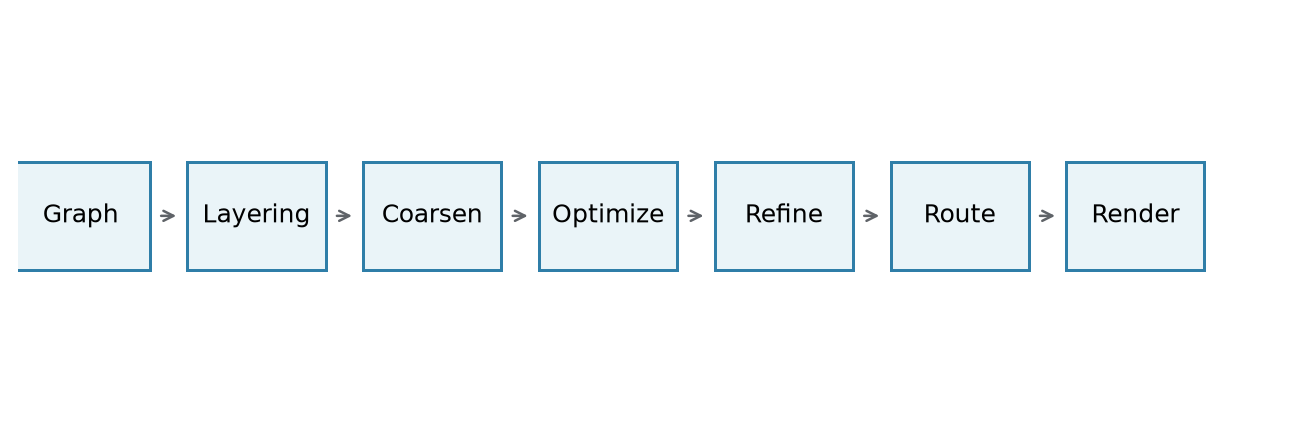
\includegraphics[width=0.92\linewidth]{figures/pipeline_stages.png}\caption{Pipeline schematic from graph construction through rendering.}\end{figure}\begin{figure}[h]\centering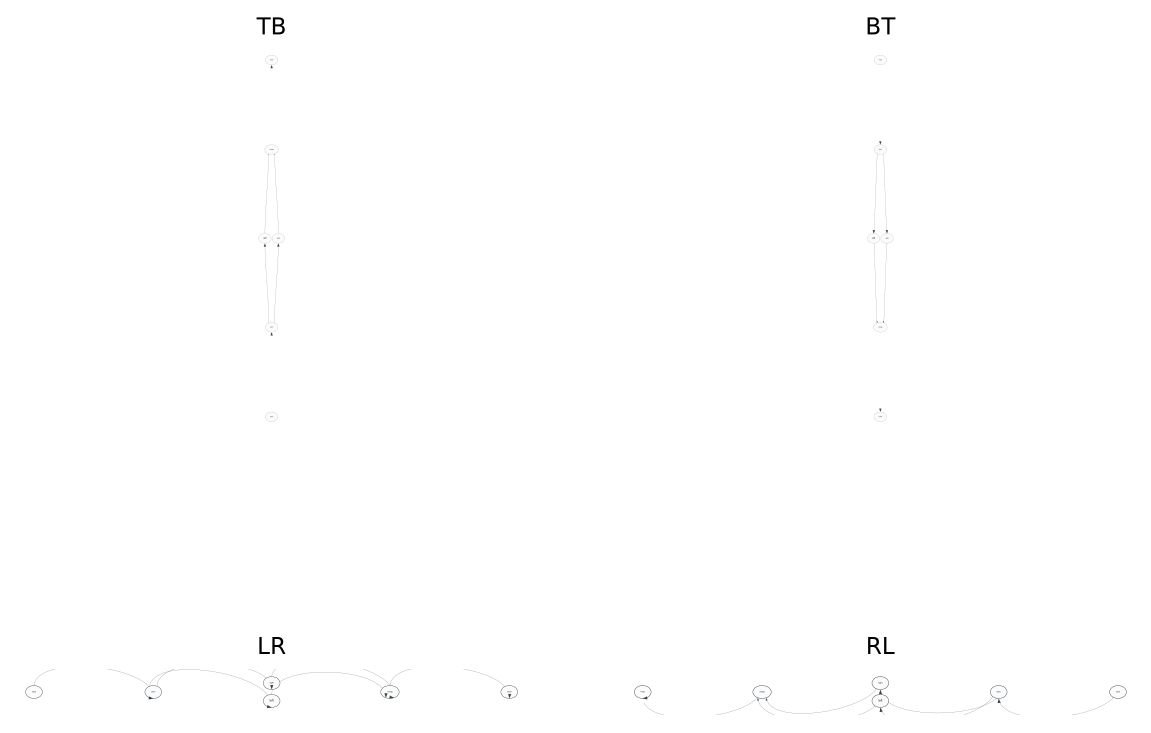
\includegraphics[width=0.92\linewidth]{figures/direction_modes.png}\caption{Direction modes change the global flow convention while preserving structure.}\end{figure}\begin{figure}[h]\centering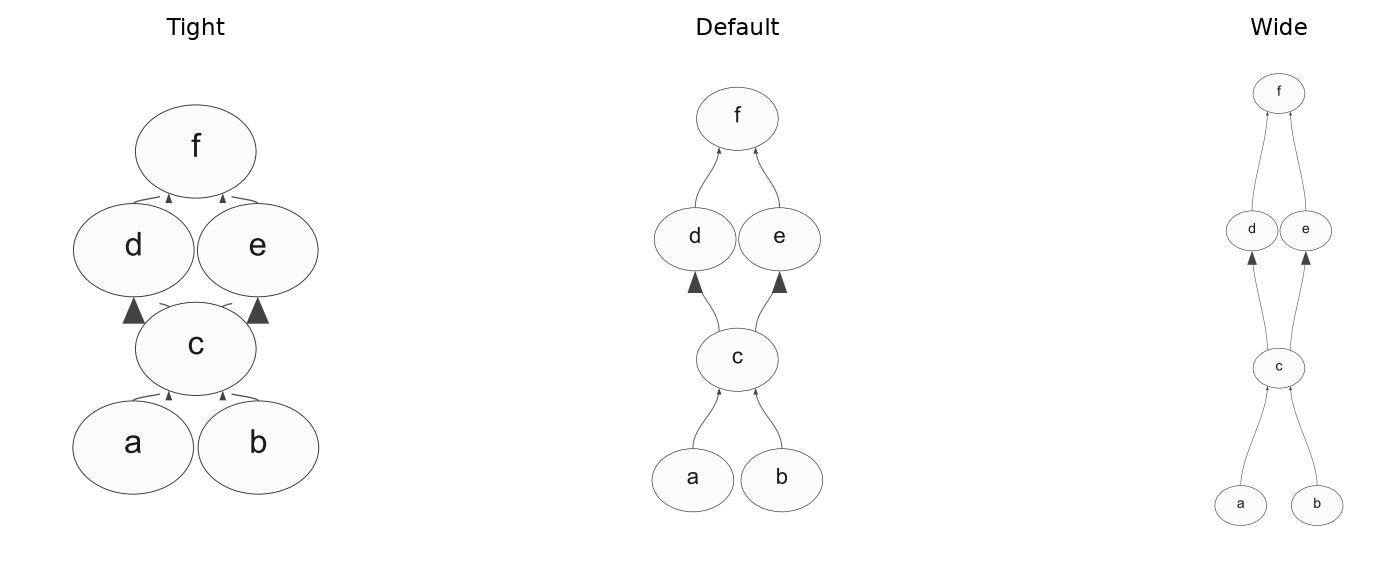
\includegraphics[width=0.92\linewidth]{figures/spacing_sweep.png}\caption{Node and rank separation alter whitespace and breathing room.}\end{figure}\begin{figure}[h]\centering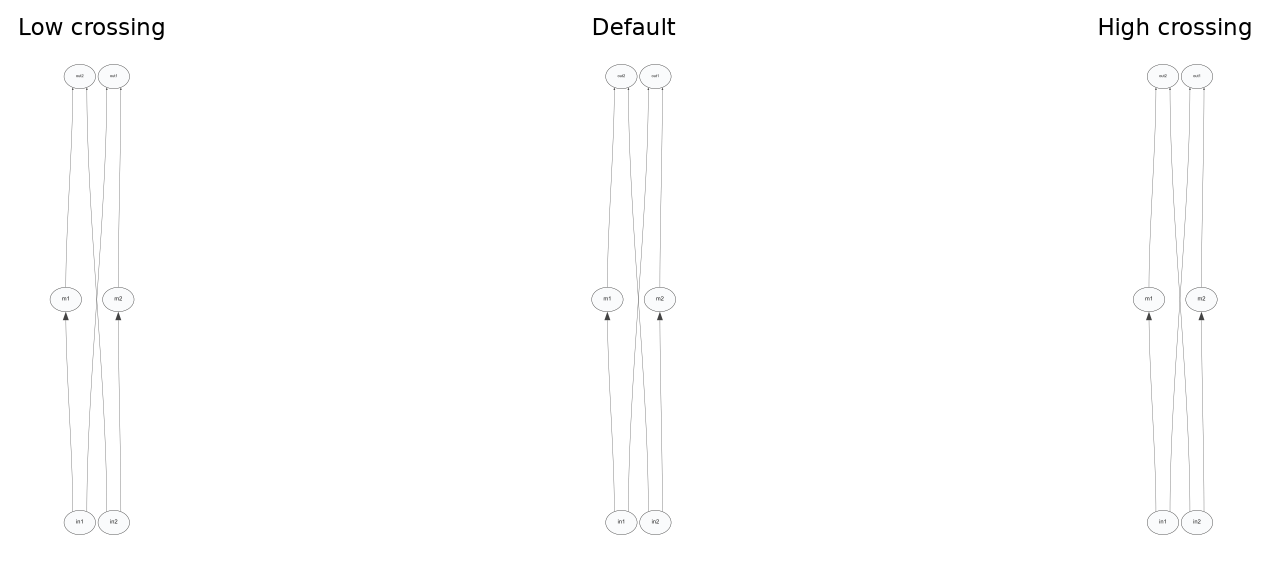
\includegraphics[width=0.92\linewidth]{figures/crossing_sweep.png}\caption{Crossing weight trades local compactness for reduced edge tangles.}\end{figure}\begin{figure}[h]\centering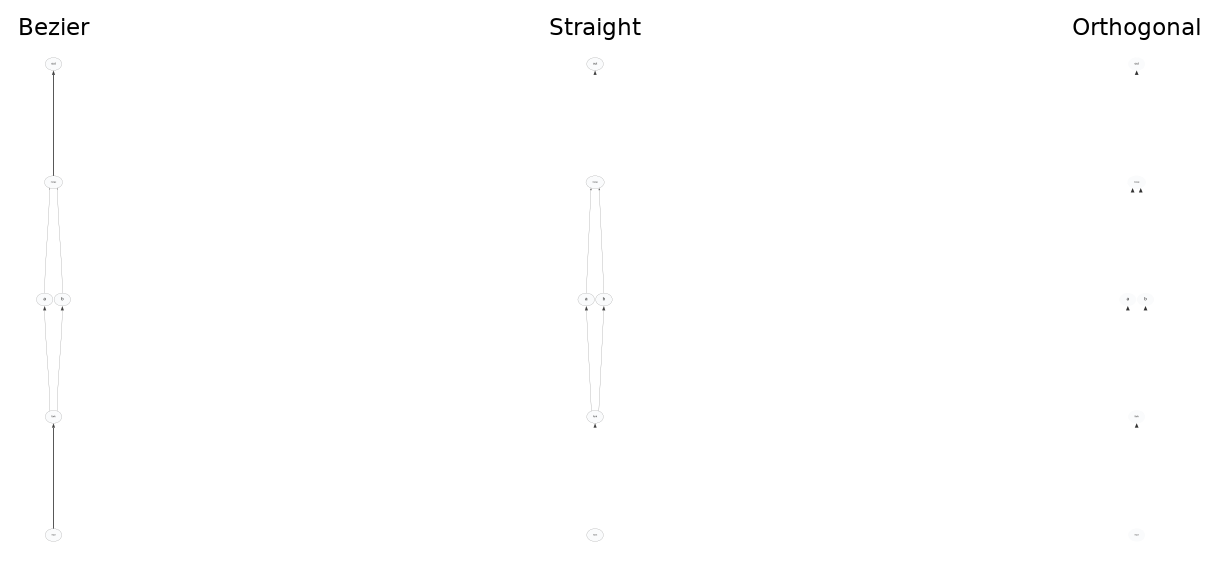
\includegraphics[width=0.92\linewidth]{figures/routing_styles.png}\caption{Edge routing style and curvature change the visual character of the same topology.}\end{figure}\begin{figure}[h]\centering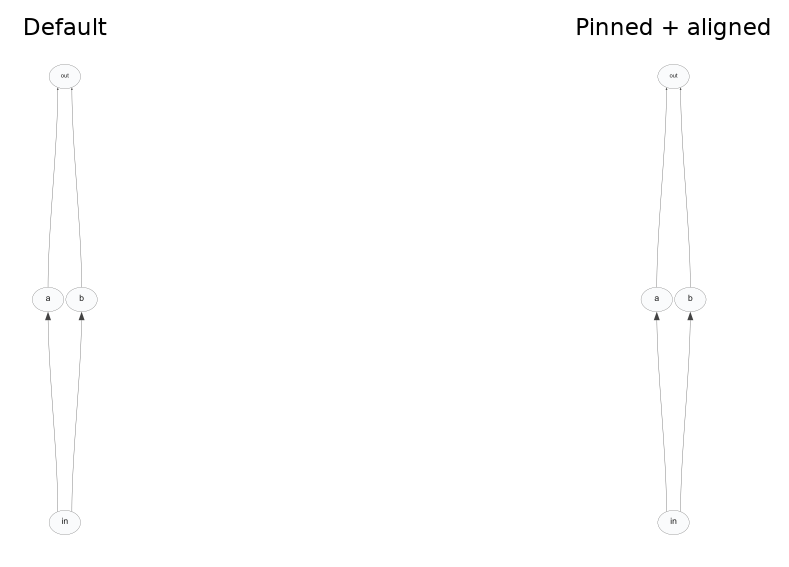
\includegraphics[width=0.92\linewidth]{figures/flex_constraints.png}\caption{Pins and alignment constraints visibly reshape the same graph.}\end{figure}
\end{document}
